%!TEX root = ../CombinatoricsNotes.tex

\section{Hypergraph Tur\'an Problems} % (fold)
\label{sec:hypergraph_turan_problems}
\marginnote{These are typically extremely difficult.}
Let $K_4^{(3)}$ be a complete 3-graph on $4$ vertices: 
\[
K_4^{(3)}=\{ \{a,b,c\},\{a,b,d\},\{a,c,d\},\{b,c,d\}\}.
\]
Then $\pi(K_4^{(3)})$ is not known\sidenote{An old and important problem.}.

Consider the generalized triangle $T_3 = \{D_1,D_2,D_3\}$ where $D_1 = \{1,2,3\}$, $D_2 = \{1,2,4\}$, and $D_3 = \{3,4,5\}$; see \cref{fig:T3}. 
\begin{marginfigure}[1cm]
\begin{center}
\begin{tikzpicture}[color=black]
\def\radius{1}


\node (a3) at (0,0){};
\node (a4) at (1,0){};
\node (a5) at (2,0) {};
\node (a2) at (.5,1) {};
\node (a1) at (.5,2) {};




\begin{scope}[fill opacity=.4]

  \filldraw[fill=red!70] ($(a1) + (0,0.15)$) 
        to[out=0,in=90] ($(a2)+(.2,0)$)
        to[out=270,in=0] ($(a3) + (0,-.15)$)
        % to[out=180,in=0] ($(a3) + (0,-.1)$)
        to[out=180,in=270] ($(a2)+(-0.2,0)$)
        to[out=90,in=180] ($(a1)+(0,.15)$);

  \filldraw[fill=blue!70] ($(a1) + (0,0.1)$) 
        to[out=0,in=90] ($(a2)+(.15,0)$)
        to[out=270,in=0] ($(a4) + (0,-.15)$)
        % to[out=180,in=0] ($(a4) + (0,-.1)$)
        to[out=180,in=270] ($(a2)+(-0.15,0)$)
        to[out=90,in=180] ($(a1)+(0,.1)$);

   \filldraw[fill=green!70] ($ (a3) + (-.2,0) $)
   		to[out=90, in=180] ($ (a4) + (0,.2) $)
   		to[out=0, in=90] ($ (a5) + (.2,0) $)
   		to[out=270, in=0] ($ (a4) + (0,-.2) $)
   		to[out=180, in=270] ($ (a3) + (-.2,0) $);


\end{scope}

\filldraw (a3) circle (\radius pt);
\filldraw (a4) circle (\radius pt);
\filldraw (a5) circle (\radius pt);
\filldraw (a2) circle (\radius pt);
\filldraw (a1) circle (\radius pt);

\end{tikzpicture}
\end{center}
\caption{An illustration of $T_3$, numbered from top to bottom, left to right. Then $D_1$ is in red, $D_2$ in blue, and $D_3$ in green. \label{fig:T3}}
\end{marginfigure}


 We will say $C: V(H) \to [k]$ is a \defn{strong $k$-coloring} if $c(v)\neq c(u)$ whenever $u$ and $v$ belong to an edge of $H$.
 $\chi_s(H) = \min k$ such that $H$ can be strongly $k$-colored.

In this language,  $\chi_s(T_3)=4$, so $T_3$ is not a subgraph of any strongly $3$-colorable graph. 
% Then density is $1\cdot\frac{2}{3}\cdot \frac{1}{3}=\frac{2}{9}$, so $\pi(T_3)\geq \frac{2}{9}$.
There exist strongly $3$-colorable graphs with density $2/9$, so $\pi(T_3)\geq 2/9$. We will show $\pi(T_3)=\frac{2}{9}$.

First, we will define an analog to the 2-graph Lagrangian defined in the previous section.
Let $H$ be an $r$-graph, $V(H) = [n]$. For $\bar x = (x_1,x_2,\dotsc,x_n)\in \R^n$, let 
\[
 P_H(\bar x) = \sum_{e\in H} \prod_{i\in e} x_i.
 \] If $x_i\geq 0$ and $\sum_i x_i = 1$, i.e. $\bar x$ corresponds to a probability distribution on $|V(H)|$, then $\frac{1}{r!}P_H(\bar x)$ is the probability that selecting $r$ verticies independently at random produces an edge. The \defn{hypergraph Lagrangian} is $\lambda(H) := \max P_H(\bar x)$ where the maximum is taken over all $\bar x \geq 0$, $\sum_{i\in[n]}x_i = 1$.

\begin{lemma} \label{lem:6p1}
Let $H$ be an $r$-graph with $|V(H)|=n$. Then
\begin{enumerate}
	\item\label{lem:6p1p1}$\lambda(H)\geq \frac{|\edges (H)|}{n^r} = P_H(\frac{1}{n}\cdot \bar 1)$.
\end{enumerate}
	Now, let $\bar x\geq 0$, $\sum_{i\in[n]}x_i = 1$ be such that $\lambda(H) = P_H(\bar x)$. Moreover, assume for every such $\bar x$, we have  $i\in[n]$, $x_i > 0$. Then,
\begin{enumerate}\setcounter{enumi}{1}
	\item\label{lem:6p1p2} For all $u,v\in V(H)$ there exists $e\in \edges (H)$  containing both $u$ and $v$, and \marginnote{That is, $H$ covers all pairs.}
	\item\label{lem:6p1p3} $\frac{\partial }{\partial x_i} P_H(\bar x) = r \cdot \lambda(H)$.

\end{enumerate}

\end{lemma}
\begin{proof}	
\begin{enumerate}
	\item This is immediate.
	\item Suppose no edge contains $u$ and $v$. Then 
	\[
	 P_H(\bar x) = C_u x_u + C_v x_v + b
	 \] 
	 where $C_u,C_v, b$ do not depend on $x_u$ and $x_v$. As in the graph case, assume $C_u\geq C_v$. Let $x'$ be such that
	 \[
	 x_u'  = x_u + x_v, \qquad x_v' = 0, \qquad x'_w = x_w \text{ for }w\neq \{u,v\}
	 \]
	 then $P_H(\bar x') \geq P_H(\bar x) = \lambda (H)$, contradicting the conditions on $H$. \marginnote{Namely that every extremal $\bar x$ has $x_v>0$.}
	 \item Lagrange multiplier principle: let $\bar x$ be a local maximum of $f(\bar x)$ such that $g(\bar x)=0$\sidenote{A constraint.}. Then 
	 \[
	 \left( \frac{\partial f}{\partial x_1}, \frac{\partial f}{\partial x_2},\dotsc, \frac{\partial f}{\partial x_n} \right) = \nabla f, \text{ and } \left( \frac{\partial g}{\partial x_1}, \dotsc, \frac{\partial g}{\partial x_n} \right) = \nabla g
	 \]
	 are colinear. Applied to $f = P_H$ and $g = \sum x_i -1$, this principle implies
	 \[
	 C = \frac{\partial P_H}{\partial x_i} = \frac{\partial P_H}{\partial x_j}
	 \]
	 for all $i,j$. Then
	 \begin{align*}	
	 \sum_{i=1}^n x_i \frac{\partial P_H}{\partial x_i} &= \sum_{i=1}^n x_i \frac{\partial}{\partial x_i}  \sum_{e\in H} \prod_{j\in e} x_j\\
	 &=\sum_{i=1}^n \sum_{e\in H} x_i   \delta_{i\in e}\prod_{j\in e\setminus \{i\}} x_j\\
	 &=\sum_{e\in H} \sum_{i=1}^n \delta_{i\in e}  \prod_{j\in e} x_j\\
	 &= \sum_{e\in H} r \prod_{j\in e} x_j
	 =r P_H(\bar x).
	 \end{align*}
	 \marginnote{This argument works for all multilinear polynomials homogeneous of degree $r$.}
	 Then
	 \[
	 C = \sum_{i=1}^n x_i C = r \lambda (H).
	 \]
\end{enumerate}
\end{proof}


Define a $3$-graph $K_4^- = \{ \{1,2,3\},\{1,2,4\},\{1,3,4\}\}$; see \cref{fig:K4minus}.
\begin{marginfigure}
\begin{center}
\begin{tikzpicture}[color=black,scale=1.5]
\def\radius{1}


\node (a3) at (0,0){};
\node (a4) at (1,0){};
\node (a2) at (.5,1) {};
\node (a1) at (.5,.5) {};

\begin{scope}[fill opacity=.4]


   \filldraw[fill=green!70] ($ (a3) + (-.1,-.1) $)
   		to[out=90, in=180] ($ (a1) + (0,.2) $)
   		to[out=0, in=90] ($ (a4) + (.1,-.10) $)
   		to[out=180, in=0] ($ (a1) + (0,-.2) $)
   		to[out=180, in=0] ($ (a3) + (-.1,-.1) $);
  \filldraw[fill=red!70] ($(a2) + (0,0.15)$) 
        to[out=0,in=90] ($(a1)+(.2,0)$)
        to[out=270,in=0] ($(a3) + (-.15,-.15)$)
        % to[out=180,in=0] ($(a3) + (0,-.1)$)
        to[out=180,in=270] ($(a1)+(-0.2,0)$)
        to[out=90,in=180] ($(a2)+(0,.15)$);


  \filldraw[fill=blue!70] ($(a2) + (0,0.1)$) 
        to[out=0,in=90] ($(a1)+(.15,0)$)
        to[out=270,in=0] ($(a4) + (.15,-.15)$)
        % to[out=180,in=0] ($(a3) + (0,-.1)$)
        to[out=180,in=270] ($(a1)+(-0.15,0)$)
        to[out=90,in=180] ($(a2)+(0,.1)$);

\end{scope}

\filldraw (a3) circle (\radius pt);
\filldraw (a4) circle (\radius pt);
\filldraw (a2) circle (\radius pt);
\filldraw (a1) circle (\radius pt);

\end{tikzpicture}
\end{center}
\caption{An illustration of $K_4^-$. \label{fig:K4minus}}
\end{marginfigure}

\begin{lemma} \label{lem:noT3noK4minus}
Let $H$ be a $3$-graph (with at least one edge) with no $T_3$ subgraph and no $K_4^-$ subgraph, then $\lambda(H) = \frac{1}{27} = \frac{2}{9}\frac{1}{3!}$.
\end{lemma}
\begin{proof}	
We may assume that any vector $\bar x$ maximizer of $P_H(\bar x)$ such that $\bar x \geq 0$, $\sum x_i = 1$ has no zero components\sidenote{Otherwise, remove those vertices; this doesn't change $P_H(\bar x)$ or $\lambda(H)$.}. Then by \cref{lem:6p1}(\ref{lem:6p1p2}), $H$ covers pairs. In fact, as $H$ contains no $T_3$ or $K_4^-$, every pair in $H$ is covered by exactly one edge. This argument is illustrated in \cref{fig:exactlyoneedge}.
\begin{marginfigure}
\begin{center}
\begin{tikzpicture}[color=black]
\def\radius{1}


\node (a3) at (0,0){};
\node (a4) at (1,0){};
% \node (a5) at (2,0) {};
\node (a2) at (.5,1) {};
\node (a1) at (.5,2) {};




\begin{scope}[fill opacity=.4]

  \filldraw[fill=red!70] ($(a1) + (0,0.15)$) 
        to[out=0,in=90] ($(a2)+(.2,0)$)
        to[out=270,in=0] ($(a3) + (0,-.15)$)
        % to[out=180,in=0] ($(a3) + (0,-.1)$)
        to[out=180,in=270] ($(a2)+(-0.2,0)$)
        to[out=90,in=180] ($(a1)+(0,.15)$);

  \filldraw[fill=blue!70] ($(a1) + (0,0.1)$) 
        to[out=0,in=90] ($(a2)+(.15,0)$)
        to[out=270,in=0] ($(a4) + (0,-.15)$)
        % to[out=180,in=0] ($(a4) + (0,-.1)$)
        to[out=180,in=270] ($(a2)+(-0.15,0)$)
        to[out=90,in=180] ($(a1)+(0,.1)$);

   % \filldraw[fill=green!70] ($ (a3) + (-.2,0) $)
   % 		to[out=90, in=180] ($ (a4) + (0,.2) $)
   % 		to[out=0, in=90] ($ (a5) + (.2,0) $)
   % 		to[out=270, in=0] ($ (a4) + (0,-.2) $)
   % 		to[out=180, in=270] ($ (a3) + (-.2,0) $);


\end{scope}

\filldraw (a3) circle (\radius pt) node[below]{$c$};
\filldraw (a4) circle (\radius pt) node[below]{$d$};
% \filldraw (a5) circle (\radius pt) node[below]{$e$};
\filldraw (a2) circle (\radius pt) node[below]{$b$};
\filldraw (a1) circle (\radius pt) node[below]{$a$};

\end{tikzpicture}
\begin{tikzpicture}[color=black]
\def\radius{1}


\node (a3) at (0,0){};
\node (a4) at (1,0){};
\node (a5) at (2,0) {};
\node (a2) at (.5,1) {};
\node (a1) at (.5,2) {};




\begin{scope}[fill opacity=.4]

  \filldraw[fill=red!70] ($(a1) + (0,0.15)$) 
        to[out=0,in=90] ($(a2)+(.2,0)$)
        to[out=270,in=0] ($(a3) + (0,-.15)$)
        % to[out=180,in=0] ($(a3) + (0,-.1)$)
        to[out=180,in=270] ($(a2)+(-0.2,0)$)
        to[out=90,in=180] ($(a1)+(0,.15)$);

  \filldraw[fill=blue!70] ($(a1) + (0,0.1)$) 
        to[out=0,in=90] ($(a2)+(.15,0)$)
        to[out=270,in=0] ($(a4) + (0,-.15)$)
        % to[out=180,in=0] ($(a4) + (0,-.1)$)
        to[out=180,in=270] ($(a2)+(-0.15,0)$)
        to[out=90,in=180] ($(a1)+(0,.1)$);

   \filldraw[fill=green!70] ($ (a3) + (-.2,0) $)
   		to[out=90, in=180] ($ (a4) + (0,.2) $)
   		to[out=0, in=90] ($ (a5) + (.2,0) $)
   		to[out=270, in=0] ($ (a4) + (0,-.2) $)
   		to[out=180, in=270] ($ (a3) + (-.2,0) $);


\end{scope}

\filldraw (a3) circle (\radius pt) node[below]{$c$};
\filldraw (a4) circle (\radius pt) node[below]{$d$};
\filldraw (a5) circle (\radius pt) node[below]{$e$};
\filldraw (a2) circle (\radius pt) node[below]{$b$};
\filldraw (a1) circle (\radius pt) node[below]{$a$};

\end{tikzpicture}

\end{center}
\caption{\emph{Left:} A depiction of two edges covering the pair $\{a,b\}$, yielding two distinct points $c$ and $d$. \emph{Right:} some edge must cover $\{c,d\}$; this edge has a third point $e$. If $e\in \{a,b\}$, then we have a $K_4^-$ subgraph; otherwise, a $T_3$ subgraph. \label{fig:exactlyoneedge}}
\end{marginfigure}
Let $|V(H)|=n$. Then, using \cref{lem:6p1}(\ref{lem:6p1p3}), we have
\[
3 n \lambda (H) = \sum_{i=1}^n \frac{\partial}{\partial x_i} P_H(\bar x) = \sum_{\{i,j\}\in [n]^{(2)}} x_i x_j \leq \lambda(K_n) = \frac{1}{2}\frac{n-1}{n}.
\]
Then
\[
\lambda(H) \leq \frac{1}{6} \frac{n-1}{n^2} \leq\frac{1}{6}\cdot\frac{2}{9}=\frac{1}{27},
\]
taking $n=3$ and using that $\frac{n-1}{n^2}$ is decreasing for $n>2$. On the other hand, by \cref{lem:6p1}(\ref{lem:6p1p1}), any $3$-graph $H$ with an edge has
\[
\lambda(H) \geq \frac{|\edges (H)|}{n^r} \geq  \frac{1}{3^3}=\frac{1}{27}.\qedhere
\]
\end{proof}

% \marginnote[1cm]{Lecture 13: Wednesday, February 17, 2016.}
\lect{2}{17}
\begin{theorem}[\cite{Erdos-Simon1983}] \label{thm:erdos_simonvits} 
Assume $\F = \{F_1,\dotsc,F_k\}$ is a family of $r$-graphs. Then for every $\epsilon$, there exists $\delta >0$ and $n_0$ such that if $G$ is an $r$-graph on $n\geq n_0$ vertices with $|\edges (G)| \geq (\pi(\F) + \epsilon) {n \choose r}$, then for some $1\leq i \leq k$, then $G$ contains at least $\delta {n\choose |V(F_i)|}$ copies of $F_i$.
\end{theorem}
We will  apply this result to $T_3$ before proving it.
\begin{theorem}
\[
\pi(T_3) = \frac{2}{9}.
\]
\end{theorem}
\begin{proof}	
Suppose $\pi(T_3) = \frac{2}{9}+ 2 \epsilon$ for some $\epsilon>0$. Let $\F = \{T_3, K_4^-\}$. Then $\pi(\F) = \frac{2}{9}$ by \cref{lem:noT3noK4minus}. Let $\delta,n_0$ satisfy \cref{thm:erdos_simonvits} for these $\F,\epsilon$. Let $G$ have $|V(G)| = n > n_0$, $|\edges (G)| \geq ( \frac{2}{9}+ \epsilon) {n \choose 3}$. We will show that (if $n$ is large enough) $G$ contains $T_3$. This will finish the proof. 

If not, then by \cref{thm:erdos_simonvits}, $G$ contains $\geq \delta {n\choose 4}$ copies of $K_4^-$. Then there exists a pair $a,b\in V(G)$ such that $a,b$ belong to $\geq \frac{\delta {n\choose 4}}{{n \choose 2}} \geq \frac{\delta}{12}n^2$ copies of $K_4^-$ in which neither $a$ nor $b$ belong to all three edges\sidenote{Why? Pigeonhole argument: we are distributing  $\delta {n\choose 4}$ copies of $K_4^-$ among ${n\choose 2}$ pairs of verticies; some pair of verticies must end up with at least $\frac{\delta {n\choose 4}}{{n \choose 2}}$ copies of $K_4^-$.}.
% \understand

Let one such copy of $K_4^-$ be that of \cref{fig:K4minuslabelled}. Then $\{a,b\}$ must belong to an edge which contains  neither $c$ nor $d$ (otherwise $\{a,b\}$ is only in two edges: $\{a,b,c\}$ and $\{a,b,d\}$).
Let $\{a,b,e\}$ be such an edge. Then $\{\{a,c,d\},\{b,c,d\},\{a,b,e\}\}$ is $T_3$ as desired. \qedhere

\begin{marginfigure}
\begin{center}
\begin{tikzpicture}[color=black,scale=1.5]
\def\radius{1}


\node (a3) at (0,0){};
\node (a4) at (1,0){};
\node (a2) at (.5,1) {};
\node (a1) at (.5,.5) {};

\begin{scope}[fill opacity=.4]


   \filldraw[fill=green!70] ($ (a3) + (-.1,-.1) $)
   		to[out=90, in=180] ($ (a1) + (0,.2) $)
   		to[out=0, in=90] ($ (a4) + (.1,-.10) $)
   		to[out=180, in=0] ($ (a1) + (0,-.2) $)
   		to[out=180, in=0] ($ (a3) + (-.1,-.1) $);
  \filldraw[fill=red!70] ($(a2) + (0,0.15)$) 
        to[out=0,in=90] ($(a1)+(.2,0)$)
        to[out=270,in=0] ($(a3) + (-.15,-.15)$)
        % to[out=180,in=0] ($(a3) + (0,-.1)$)
        to[out=180,in=270] ($(a1)+(-0.2,0)$)
        to[out=90,in=180] ($(a2)+(0,.15)$);


  \filldraw[fill=blue!70] ($(a2) + (0,0.1)$) 
        to[out=0,in=90] ($(a1)+(.15,0)$)
        to[out=270,in=0] ($(a4) + (.15,-.15)$)
        % to[out=180,in=0] ($(a3) + (0,-.1)$)
        to[out=180,in=270] ($(a1)+(-0.15,0)$)
        to[out=90,in=180] ($(a2)+(0,.1)$);

\end{scope}

\filldraw (a3) circle (\radius pt) node[below] {a};
\filldraw (a4) circle (\radius pt) node[below] {b};
\filldraw (a2) circle (\radius pt) node[below]{d};
\filldraw (a1) circle (\radius pt) node[below]{c};

\end{tikzpicture}
\end{center}
\caption{A labelled illustration of $K_4^-$. \label{fig:K4minuslabelled}}
\end{marginfigure}

\end{proof}


\begin{proof}[Proof of \cref{thm:erdos_simonvits}]
Let us only consider the case $\F=\{F\}$ for simplicity. Let $n'$ be such that every graph $G$ on $n'$ vertices with $|\edges(G)|\geq (\pi (\F) + \frac{\epsilon}{2}) {n' \choose r}$ contains $F$; such an $n'$ exists by the definition of limit. We will choose $n_0$ appropriately large compared to $n'$.
% \unsure{Can't we have any $n_0\geq n'$?}
\begin{claim}
At least $\frac{\epsilon}{2}{n\choose n'}$ subgraphs of $G$ on $n'$ vertices have at least $(\pi(F) + \frac{\epsilon}{2} ) {n' \choose r}$ edges, and thus have a copy of $F$.
\end{claim}
\begin{subproof}[Proof of claim.]
Suppose not. (Let $V(G)=[n]$). Then
\begin{gather*}
|\edges(G)| \underbrace{{n-r \choose n'-r}}_{\substack{\text{\# of $n'$-element sets}\\\text{containing an edge}}} = \sum_{X\in [n]^{(n')}} \underbrace{| \edges (G|X)|}_{\text{edges in $G$ restricted to $X$}}
\end{gather*}
\begin{fullwidth}
By our assumption,
\begin{align*}
\sum_{X\in [n]^{(n')}} | \edges (G|X)| &= \sum_{X:\, |\edges (X)| \geq ( \pi(F) + \frac{\epsilon}{2}) {n' \choose r}) }\edges (G|X) + \sum_{X:\, |\edges (X)| < ( \pi(F) + \frac{\epsilon}{2}) {n' \choose r}) }\edges (G|X) \\
&\leq\frac{\epsilon}{2} {n \choose n'}\underbrace{{n' \choose r}}_{\text{maximal \# edges}} + (1 - \frac{\epsilon}{2}){n \choose n'} (\pi(\F) + \frac{\epsilon}{2}){n' \choose r}
\end{align*}
On the other hand, $|\edges (G)| \geq ( \pi(F) + \epsilon) {n \choose r})$, so we have
\[
( \pi(F) +\epsilon) {n \choose r}{n-r \choose n'-r}\leq \frac{\epsilon}{2} {n \choose n'}{n' \choose r} + (1 - \frac{\epsilon}{2}){n \choose n'} (\pi(\F) + \frac{\epsilon}{2}){n' \choose r}.
\]
\end{fullwidth}
But, by \cref{eq:binomial_identity_boxes}, we have ${n \choose r}{n-r \choose n'-r}  ={n \choose n'}{n' \choose r} $, so
\begin{gather*}	
\pi(F) + \epsilon \leq \frac{\epsilon}{2} + (1- \frac{\epsilon}{2}) (\pi(F) + \frac{\epsilon}{2})\\
\pi(F)+\frac{\epsilon}{2} \leq \pi(F) + \frac{\epsilon}{2} - \frac{\epsilon}{2}\pi(F) - \frac{\epsilon^2}{4}\\
0 \leq - \frac{\epsilon}{2}\pi(F) - \frac{\epsilon^2}{4}
\end{gather*}
which is a contradiction, since $\pi(F)\geq 0$.
\end{subproof}
So by the choice of $n'$ each of these subgraphs contains $F$. Suppose $G$ contains $k$ copies of $F$, and $v = |V(F)|$. Then each of these copies is counted in ${n-v \choose n'-v}$ many $n'$-vertex subgraphs. So, by our claim, $k {n-v \choose n'-v} \geq \frac{\epsilon}{2}{n\choose n'}$. Then,
\[
k\geq \frac{\epsilon}{2} \frac{{n\choose n'}}{{n-v\choose n'-v}} = \frac{\epsilon}{2} \frac{{n\choose v}}{{n' \choose v}} = \frac{\frac{\epsilon}{2}}{{n' \choose v}} {n \choose v} = \delta {n \choose v}
\]
where $\delta := \frac{\frac{\epsilon}{2}}{{n' \choose v}}$, and we've used \cref{eq:binomial_identity_boxes} again.
\end{proof}


\subsection{Tur\'an density of Fano plane.} \marginnote{Finite projective geometry}
The Fano plane $F_7$ is the 3-graph on vertices $\Z_2^3 \setminus \{(0,0,0)\}$, i.e. triples of 0s and 1s not all zero. We declare $\{x,y,z\}$ to be an edge of $F_7$ if $x+y+z = 0 \iff x+y=z$; see \cref{fig:Fano} for an illustration. Note there are seven edges.
\begin{marginfigure}
\begin{center}
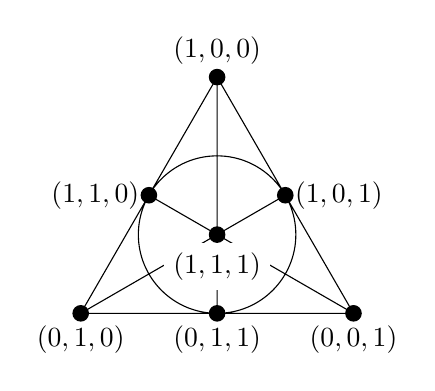
\begin{tikzpicture}
  \draw (30:1)  -- (210:2)
        (150:1) -- (330:2)
        (270:1) -- (90:2)
        (90:2)  -- (210:2) -- (330:2) -- cycle
        (0:0)   circle (1);
  \fill (0:0)   circle(3pt) node[below,fill=white,yshift=-3pt,xshift=0pt]{$(1,1,1)$}
        (30:1)  circle(3pt) node[right]{$(1,0,1)$}
        (90:2)  circle(3pt) node[above,yshift=1pt,xshift=0pt]{$(1,0,0)$}
        (150:1) circle(3pt) node[left]{$(1,1,0)$}
        (210:2) circle(3pt) node[below,yshift=-1pt]{$(0,1,0)$}
        (270:1) circle(3pt) node[below,yshift=-1pt]{$(0,1,1)$}
        (330:2) circle(3pt) node[below,yshift=-1pt]{$(0,0,1)$};
\end{tikzpicture}
\end{center}
\caption{A depiction of the Fano plane $F_7$. Each straight line is an edge, and the circle is an edge; each edge contains exactly 3 vertices, since $F_7$ is a 3-graph.} \label{fig:Fano}
\end{marginfigure}


Recall that $c: V(H)\to [k]$ is a $k$-coloring of a hypergraph $H$ if no edge of $H$ is monochromatic, and $\chi(H)$ is the minimum $k$ such that $H$ admits a $k$-coloring. We have the following lemma.
\begin{lemma} \label{lem:chiF7}
\[	
\chi(F_7) = 3.
\]
\end{lemma}
\begin{proof}	
In a random $3$-coloring, the probability that an edge is monochromatic is $\frac{1}{9}$, so the expected number of monochromatic edges is $\frac{7}{9}<1$. So there exists a 3-coloring with no monochromatic edges. So $\chi(H) \leq 3$.

Suppose there exists a 2-coloring of $F_7$. Then by pigeonhole, at least four vertices have to recieve the same color; say $w,x,y,z$, say with color 1. Since $\{x,y,x+y\}$ is an edge: $x+y+x+y = 2x+2y = 0$, we must have $x+y$ be color 2; similarly with $y+z$ and $x+z$. But then $\{x+y,y+z,x+z\}$ is a monochromatic edge, of color 2.
\end{proof}

\begin{marginfigure}
\begin{center}
\begin{tikzpicture}[color=black,scale=1.2]
\def\radius{1}

\node at (-.5, 1.7) {\small $\tfrac{n}{2}$};

\node at (-.5, .3)  {\small $\tfrac{n}{2}$};

\draw[dashed] (-.7,1) -- (2.3,1);
\begin{scope}
\node (a3) at (0,0){};
\node (a4) at (1,0){};
% \node (a5) at (2,0) {};
\node (a2) at (.5,1) {};
\node (a1) at (.5,2) {};
\begin{scope}[fill opacity=.4]


  \filldraw[fill=green!70] ($(a1) + (.3,0.2)$) 
        to[out=0,in=90] ($(a2)+(.3,0)$)
        to[out=270,in=0] ($(a4) + (0,-.15)$)
        % to[out=180,in=0] ($(a4) + (0,-.1)$)
        to[out=180,in=270] ($(a2)+(-0.15,0)$)
        to[out=90,in=180] ($(a1)+(0,.2)$) -- cycle;


  \filldraw[fill=red!70] ($(a1) + (0,0.15)$) 
        to[out=0,in=90] ($(a2)+(.2,0)$)
        to[out=270,in=0] ($(a3) + (0,-.15)$)
        % to[out=180,in=0] ($(a3) + (0,-.1)$)
        to[out=180,in=270] ($(a2)+(-0.3,0)$)
        to[out=90,in=180] ($(a1)+(0,.15)$);


\end{scope}

\filldraw (a3) circle (\radius pt) node{};
\filldraw ($(a3) +(.2,.3)$) circle (\radius pt) node{};

\filldraw (a4) circle (\radius pt) node{};
\filldraw (a1) circle (\radius pt) node{};
\filldraw ($(a1) + (.33,.05)$) circle (\radius pt) node{};

\end{scope}

\begin{scope}[xshift=1.5cm,yshift=2cm,rotate=180]
\node (a3) at (0,0){};
\node (a4) at (1,0){};
% \node (a5) at (2,0) {};
\node (a2) at (0,1) {};
\node (a1) at (0,2) {};
\begin{scope}[fill opacity=.4]

  \filldraw[fill=blue!70] ($(a1) + (0,0.15)$) 
        to[out=0,in=90] ($(a2)+(.2,0)$)
        to[out=270,in=0] ($(a3) + (0,-.15)$)
        % to[out=180,in=0] ($(a3) + (0,-.1)$)
        to[out=180,in=270] ($(a2)+(-0.2,0)$)
        to[out=90,in=180] ($(a1)+(0,.15)$);


\end{scope}

\filldraw (a3) circle (\radius pt) node{};
% \filldraw (a4) circle (\radius pt) node{};
\filldraw (a1) circle (\radius pt) node{};
\filldraw ($(a3) +(.1,.3)$) circle (\radius pt) node{};

\end{scope}

\end{tikzpicture}
\end{center}
\caption{A $3$-graph on $n$ verticies formed by partitioning the verticies in two approximately equal parts, and choosing edges as all triples with at least one vertex in each part. For clarity, not all the edges are drawn here.} \label{fig:3graph_one_from_each}
\end{marginfigure}
If we partition $n$ verticies into two approximately equal halves, we may define a $3$-graph by declaring all triples with at least one member in each half to be edges; see \cref{fig:3graph_one_from_each} for an illustration.
There are $\frac{3}{4}{n\choose 3} + O(n^2)$ edges in this graph. If this graph had a Fano plane subgraph, then we could 2-color the Fano plane, which is impossible by \cref{lem:chiF7}. Thus, the graph of \cref{fig:3graph_one_from_each} must not have an $F_7$ subgraph, so $\pi(F_7)\geq \frac{3}{4}$.
%  We see that this is impossible by first considering the triangle (verticies $\{a,w,c\}$ in \cref{fig:fano_labelled}); if those three verticies were monochromatic red, then the circle $\{b,y,z\}$ must be monochromatic blue (or else one of the sides of the triangle would be monochromatic red). In either case, if the Fano plane were 2-colorable, then one vertex of the triangle must be a different color than the other two. Let's say $a$ is red, while $w$ and $c$ are blue. Then $z$ must be red or else $\{c,z,w\}$ would be monochromatic blue. Since $\{a,x,z\}$ is an edge, $x$ must be blue. For $\{b,x,w\}$ and $\{c,x,y\}$ to not be monochromatic blue  edges, both $b$ and $y$ must be red. This yields $\{b,y,z\}$ as a monochromatic red edge.
% \begin{marginfigure}
% \begin{center}
% \begin{tikzpicture}
% \def\radius{2}
% \def\shift{1}
%   \draw (30:1)  -- (210:2)
%         (150:1) -- (330:2)
%         (270:1) -- (90:2)
%         (90:2)  -- (210:2) -- (330:2) -- cycle
%         (0:0)   circle (1);
%   \fill[blue] (0:0)   circle(\radius pt) node[left,yshift=0pt,xshift=-3pt](x){$x$};
%   \fill      (30:1)  circle(\radius pt) node[right,xshift=\shift pt](y){$y$};
%   \fill[red]     (90:2)  circle(\radius pt) node[above,yshift=\shift pt,xshift=0pt](a){$a$};
%   \fill      (150:1) circle(\radius pt) node[left, xshift=-\shift pt](b){$b$};
%   \fill[blue]      (210:2) circle(\radius pt) node[left,yshift=0pt, xshift=-\shift pt](c){$c$};
%   \fill[red]      (270:1) circle(\radius pt) node[below,yshift=-\shift pt](z){$z$};
%   \fill[blue]      (330:2) circle(\radius pt) node[below,yshift=-\shift pt](w){$w$};
%   %   \draw[blue] (0:0) -- (30:1) node[midway,above]{$L_c$}
%   %         (270:1) -- (330:2) ;
%   %   \draw[red!30]
%   %       (270:1) -- (0:0) node[midway,left]{$L_a$}
%   %       (30:1) -- (330:2);
%   %   % \draw[green]
%   %     % (270:1) -- ;
%   % \draw[green] (270:1) arc (270:270+120:1);
%   % \draw[green] (0:0) -- (330:2) node[near start]{$L_b$} ;
% \end{tikzpicture}
% \end{center}
% \caption{A depiction of the proof to show that the Fano plane is impossible to 2-color. } \label{fig:fano_labelled}
% \end{marginfigure}

% \missingfigure{Partition vertices into two parts of size $\sim \frac{n}{2}$, and take all edges which have $\geq 1$ vertex in each part. This hypergraph contains $\sim \frac{3}{4}{n\choose 3}$ edges, so $\pi(F_7) \geq \frac{3}{4}$.}
\begin{theorem}[\cite{DeCaenFuredi}] 
\[	
\pi(F_7) = \frac{3}{4}.
\]
\end{theorem}
\begin{proof}	
Suppose not: $\pi(F_7) = \frac{3}{4}+ 2 \epsilon$ for some $\epsilon>0$. By \cref{lem:subgraph_with_min_vertex_degree},  for every $n_0$ there exists a $3$-graph $G$ on $n\geq n_0$ vertices with no $F_7$ subgraph such that every vertex of $G$ belongs to $\geq ( \frac{3}{4} + \epsilon) {n\choose 2}$ edges. Moreover, we may assume that $G$ contains $K_4^{(3)}$: four vertices such that every triple forms an edge\sidenote{If not, every set of four verticies yields at most three edges, which implies $G$ has at most $\frac{3}{4}{n\choose 2}$ edges in total, contradicting our assumption.}.
% \unsure{why can we do this?}
 We'll take these vertices to be $a,b,c,d$.
% \marginnote{Lecture 14: Wednesday, February 24, 2016.}
\lect{2}{24}

For $x\in V(G)$, let $L_x = \{ \{y,z\}: \{x,y,z\} \in \edges (G) \}$. This is called the \defn{link graph} of $x$ in $G$.
For $x_1,x_2,\dotsc,x_k$ we will consider $L_{x_1} \cup L_{x_2} \cup \dotsm \cup L_{x_k}$ (abusing notation) as a \defn{multigraph}, meaning that we count multiplicity.

\begin{claim}
If $\{a,b,c\}\in \edges (G)$, then $L_a \cup L_b\cup L_c$ induces at most 15 edges (counting multiplicity) on any four vertices. \marginnote{A single link graph can induce ${4 \choose 2} = 6$ edges on four vertices, so our naive bound is 18. Our claim is that this additional structure of being link graphs of $G$ lets us do slightly better.}
\end{claim}



\begin{marginfigure}
\begin{center}
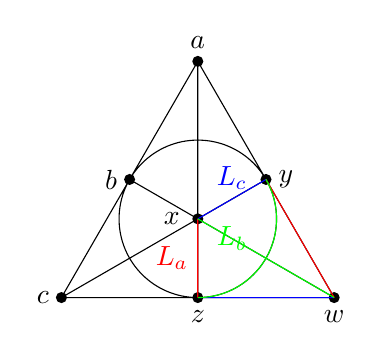
\begin{tikzpicture}
\def\radius{2}
\def\shift{1}
  \draw (30:1)  -- (210:2)
        (150:1) -- (330:2)
        (270:1) -- (90:2)
        (90:2)  -- (210:2) -- (330:2) -- cycle
        (0:0)   circle (1);
  \fill (0:0)   circle(\radius pt) node[left,yshift=0pt,xshift=-3pt](x){$x$}
        (30:1)  circle(\radius pt) node[right,xshift=\shift pt](y){$y$}
        (90:2)  circle(\radius pt) node[above,yshift=\shift pt,xshift=0pt](a){$a$}
        (150:1) circle(\radius pt) node[left, xshift=-\shift pt](b){$b$}
        (210:2) circle(\radius pt) node[left,yshift=0pt, xshift=-\shift pt](c){$c$}
        (270:1) circle(\radius pt) node[below,yshift=-\shift pt](z){$z$}
        (330:2) circle(\radius pt) node[below,yshift=-\shift pt](w){$w$};
    \draw[blue] (0:0) -- (30:1) node[midway,above]{$L_c$}
    			(270:1) -- (330:2) ;
   	\draw[red]
   			(270:1) -- (0:0) node[midway,left]{$L_a$}
   			(30:1) -- (330:2);
   	% \draw[green]
   		% (270:1) -- ;
	\draw[green] (270:1) arc (270:270+120:1);
	\draw[green] (0:0) -- (330:2) node[near start]{$L_b$} ;
\end{tikzpicture}
\end{center}
\caption{%The Fano plane, labelled, with the complete 2-graph on $\{x,y,z,w\}$ colored. 
Given an edge $\{a,b,c\}$, we consider any four vertices $x,y,z,w \in L_a\cup L_b\cup L_c$, and on these seven vertices, we construct the Fano plane. Since $G$ contains no $F_7$ subgraph, the edges drawn here must not all appear in the link graphs.\label{fig:fano_link_graphs}}
\end{marginfigure}
\begin{subproof}[Proof of claim.]	

Let $x,y,z,w$ be vertices in $V(G) \setminus \{a,b,c\}$. As $G$ contains no $F_7$, there does not exist a partition of the edge set of the complete 2-graph on $\{x,y,z,w\}$ into three subsets $M_1,M_2,$ and $M_3$ of size two such that  $|M_1\cap L_a|=2, |M_2\cap L_b|=2,$ and $|M_3\cap L_c|=2$; see \cref{fig:fano_link_graphs}. 

Suppose $L_a\cup L_b\cup L_c$ has $\geq 16$ edges on $\{x,y,z,w\}$, i.e., these link graphs missed at most 2 out of the maximum possible number of edges (which is $3*{4\choose 2} = 18$, recalling that we count edges in the link graphs with multiplicity).
Let 
\begin{align*}	
M_1 &=\{ \{x,y\}, \{z,w\} \}, &
M_2 &= \{ \{ x,w \}, \{ y,z \} \}, &
M_3 &=\{ \{x,z\}, \{ y,w \} \}
\end{align*}
as shown in \cref{fig:complete_graph_in_links_fano}. 
Up to changing the labels, there are two cases.
\begin{marginfigure}
\begin{center}
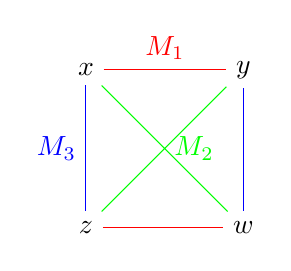
\begin{tikzpicture}[scale=2]
\node (x) at (0,1) {$x$};
\node (y) at (1,1) {$y$};

\node (z) at (0,0) {$z$};

\node (w) at (1,0) {$w$};

\draw[green] (x) -- (w) node[midway,right]{$M_2$}
			(y) -- (z);

\draw[blue]
			(x) -- (z) node[midway,left]{$M_3$}
			(y) -- (w);

\draw[red]
			(x) -- (y) node[midway,above]{$M_1$}
			(z) -- (w);

\end{tikzpicture}	
\end{center}
\caption{A choice of partition $M_1,M_2,M_3$ of edges of the complete graph on  $\{x,y,z,w\}$, chosen to correspond to \cref{fig:fano_link_graphs}.  \label{fig:complete_graph_in_links_fano}}
\end{marginfigure}
\begin{enumerate}[{Case }1:]
	\item  Both missing edges belong to $M_1$. That is, either for some $x\in \{a,bc\}$, we have $|L_x\cap M_1| = 0$ or for some $x,y\in \{a,b,c\}$ distinct, we have $|L_x\cap M_1| = 1$ and $|L_y\cap M_1| = 1$.

  In any case, $M_1$ fully intersects with one of the $L_x$; say, $L_a$ (that is, $|L_a\cap M_1|= 2$). Then since those were the only two missing edges, we have $|L_b\cap M_2| = |L_c\cap M_3|=2$. 
   % Then wlog $M_1\subset L_a$, $M_2\subset L_b$, $M_3\subset L_c$. ($M_1$ belongs to one link graph).
	\item One missing edges belongs to $M_1$ and one $M_2$. That is, $|M_1\cap L_x| = 1$ and $|M_2\cap L_y| = 1$, for some $x,y\in\{a,b,c\}$. Since those were the only missing edges, $M_1$ fully intersects with two link graphs, and $M_2$ with two. So we may choose them to be different, putting, say, $|M_1\cap L_a|=2$, $|M_2\cap L_b|=2$, and $|M_3\cap L_c|=2$.\qedhere
  % As before, for some $x$, we still have $|M_1\cap L_x| = 2$
  % Then wlog $M_1\subset L_a$ (belongs to 2 link graphs), $M_2\subset L_b$ ($M_2$ belongs to 1 link graph not $L_a$), and $M_3\subset L_c$.
\end{enumerate}
\end{subproof}

\begin{claim}
If $a,b,c,d$ are the vertices of $K_4^{(3)}$, then $L_a\cup L_b\cup L_c\cup L_d$ induces at most 20 edges counted with multiplicies in $V(G)\setminus \{a,b,c,d\}$.
\end{claim}
\begin{subproof}	
Apply previous claim to all 4 edges $\{a,b,c\}$, $\{a,b,d\}$, $\{a,c,d\}$, $\{b,c,d\}$. In total, the resulting multigraph will have at most 60 edges but each $L_i$ (for $i\in \{a,b,c,d\}$) is counted 3 times.
\end{subproof}

Then,
\[
|L_a \cup L_b\cup L_c \cup L_d| \geq (3 + \epsilon) {n \choose 2}
\]
If we restrict to $L_a\cup L_b\cup L_c\cup L_d$ to $V(G)\setminus \{a,b,c,d\}$, we still have at least 
\begin{equation} \label{eq:numedges} \tag{$\star$f}
(3+ \epsilon){n\choose 2} - 12n
\end{equation}
 edges, where we've overcounted edges in $L_a\cup L_b\cup L_c\cup L_d$ using one of $\{a,b,c,d\}$.

\marginnote{Note in the following, we are considering $2$-graphs.}
We may think of a multigraph with vertex set $V$ as a function $w: V^{(2)} \to \Z_+$.
Let $m(n,k,r)$ be the maximum number of edges (the sum of weights $\sum_{e\in V^{(2)}} w(e)$) in a multigraph on $n$ vertices such that any $k$ vertices induce $\leq r$ edges.
We will show that 
\begin{equation} \label{eq:max_multigraph_edges} \tag{$\star$}
m(n,4,20) \leq 3 {n\choose 2} + n -2
\end{equation}
for $n\geq 4$. This will finish the proof, as it contradicts (\ref{eq:numedges}) for large $n$.
We will assume 
\begin{equation} \label{eq:assumption_for_max_multigraph} \tag{$\star\star$}
m(n,3,10) \leq 3 {n\choose 2} + n-2.
\end{equation}
The proof of this is left as an exercise.
Let us prove (\ref{eq:max_multigraph_edges}) by induction.
Base case: 
\[
m(4,4,20) \leq 3\cdot 6 + 4-2 = 20.
\]
Induction step: Using (\ref{eq:assumption_for_max_multigraph}), we assume $\{a,b,c\} \subset V$  induces $k\geq 11$ edges. Let $w(x)= \sum_{e\ni x} w(e)$ for $x\in \{a,b,c\}$.
Then
\begin{align*}	
w(a) +w(b) + w(c) &= \underbrace{2k}_{\substack{\text{weight of edges} \\ \text{ with two of $\{a,b,c\}$}}} + \sum_{z\in V\setminus \{a,b,c\}} ( w(za) + w(zb) + w(zc))
\end{align*}
 Since every four verticies span at most 20 edges, for each $z\in V\setminus \{a,b,c\}$ we have $w(za) +w(zb) + w(zc)  \leq 20-k$.  Then 
\begin{align*}
w(a) + w(b)+ w(c) &\leq
2k + (n-3) (20-k) \\
&= 20(n-3) - k(n-5)\\
&\leq 20 (n-3) - 11(n-5) = 9n-5
\end{align*}
WLOG, $w(a) \leq 3n-2$ by pigeonhole.
By the induction hypothesis, $V\setminus \{a\}$ induces total weight at most
\[
3 {n-1 \choose 2} + (n-1)-2.
\]
So the total number of edges is at most
\[
 3 {n-1 \choose 2} + (n-1)-2 + (3n-2) \leq 3 {n\choose 2} + n-2. \qedhere
\]
\end{proof}
% section hypergraph_turan_problems (end)
